\documentclass{article}

\documentclass{article}

\usepackage{amsmath, amsthm, amssymb, amsfonts}
\usepackage{thmtools}
\usepackage{graphicx}
\usepackage{setspace}
\usepackage{geometry}
\usepackage{float}
\usepackage{hyperref}
\usepackage[utf8]{inputenc}
\usepackage[english]{babel}
\usepackage{framed}
\usepackage[dvipsnames]{xcolor}
\usepackage{tcolorbox}

\colorlet{LightGray}{White!90!Periwinkle}
\colorlet{LightOrange}{Orange!15}
\colorlet{LightGreen}{Green!15}

\newcommand{\HRule}[1]{\rule{\linewidth}{#1}}


\begin{document}

\title{ \normalsize \textsc{}
		\\ [2.0cm]
		\HRule{1.5pt} \\
		\LARGE \textbf{\uppercase{Processing point clouds
}
		\HRule{2.0pt} \\ [0.6cm] \LARGE{GEO1015 assignment 4} \vspace*{10\baselineskip}}
		}
\date{}
\author{\textbf{Authors} \\ 
            Lars Boertjes \t 4704541 \\ 
		  Noah Alting \t 4828968 \\
            Marieke van Arnhem \t 4918738 \\ 
            \\
		\textbf{TU Delft} \\
		\today}

\maketitle

\newpage

\tableofcontents
\newpage

% ------------------------------------------------------------------------------
% Introduction
% ------------------------------------------------------------------------------

\section{Introduction}

This document provides an overview of our workflow to Assignment 4, focusing on the processing of a point cloud to a Canopy Height Model (CHM). Our point cloud source is a designated tile, specifically tile 69BZ2\_13 from the AHN4 dataset. For a more manageable dataset, we extracted a 500x500 meter clip from this tile. The processing pipeline involved extracting ground points and generating a gridded Digital Terrain Model (DTM), identifying vegetation points and creating a grid, and ultimately producing a Canopy Height Model (CHM).

This report will guide you through the steps we took to create a Canopy Height Model from the AHN4 point cloud dataset.
\newpage

\section{Pick a Team and Assign AHN4 Tile}
\newpage


\section{Download and Prepare the Dataset}

For Assignment 4, we focused on processing a point cloud derived from the designated tile 69BZ2\_13 obtained from GeoTiles in LAS format. This tile covers the small village of Scheulder in Limburg. Figure \ref{fig:full_tile} displays the full tile seen from above using CloudCompare.

\begin{figure}[h]
  \centering
  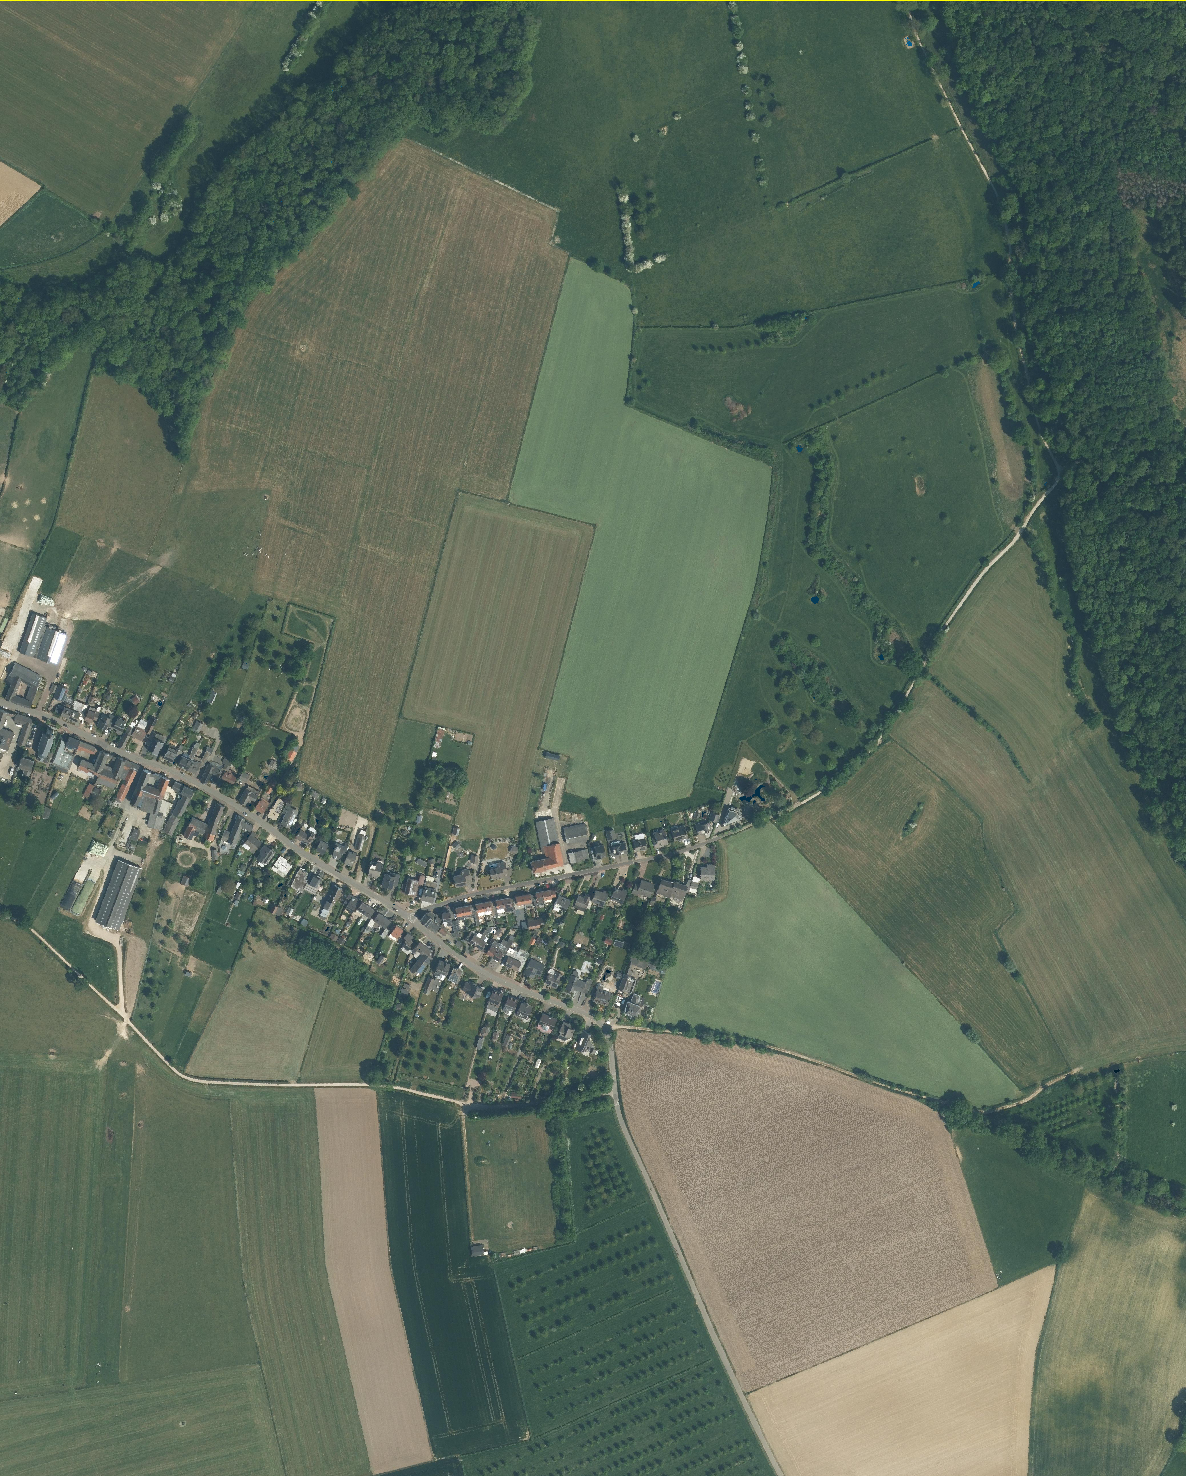
\includegraphics[width=0.5\linewidth]{img/screenshot_full_tile.png}
  \caption{Full tile view in CloudCompare.}
  \label{fig:full_tile}
\end{figure}

For more convenient processing and as stated in the assignment, we reduced the full tile to a 500x500 meter clipped tile, shown in Figure \ref{fig:cropped_front}. This clipped tile features buildings, forests, water bodies, and also some elevation. In the figure, the clipped tile can be seen as all the points with RGB coloring. The start tile has been colored using a gray scale for the intensity values. This is done to give an indication of the placement of the clipped tile within its context. 

\begin{figure}[h]
  \centering
  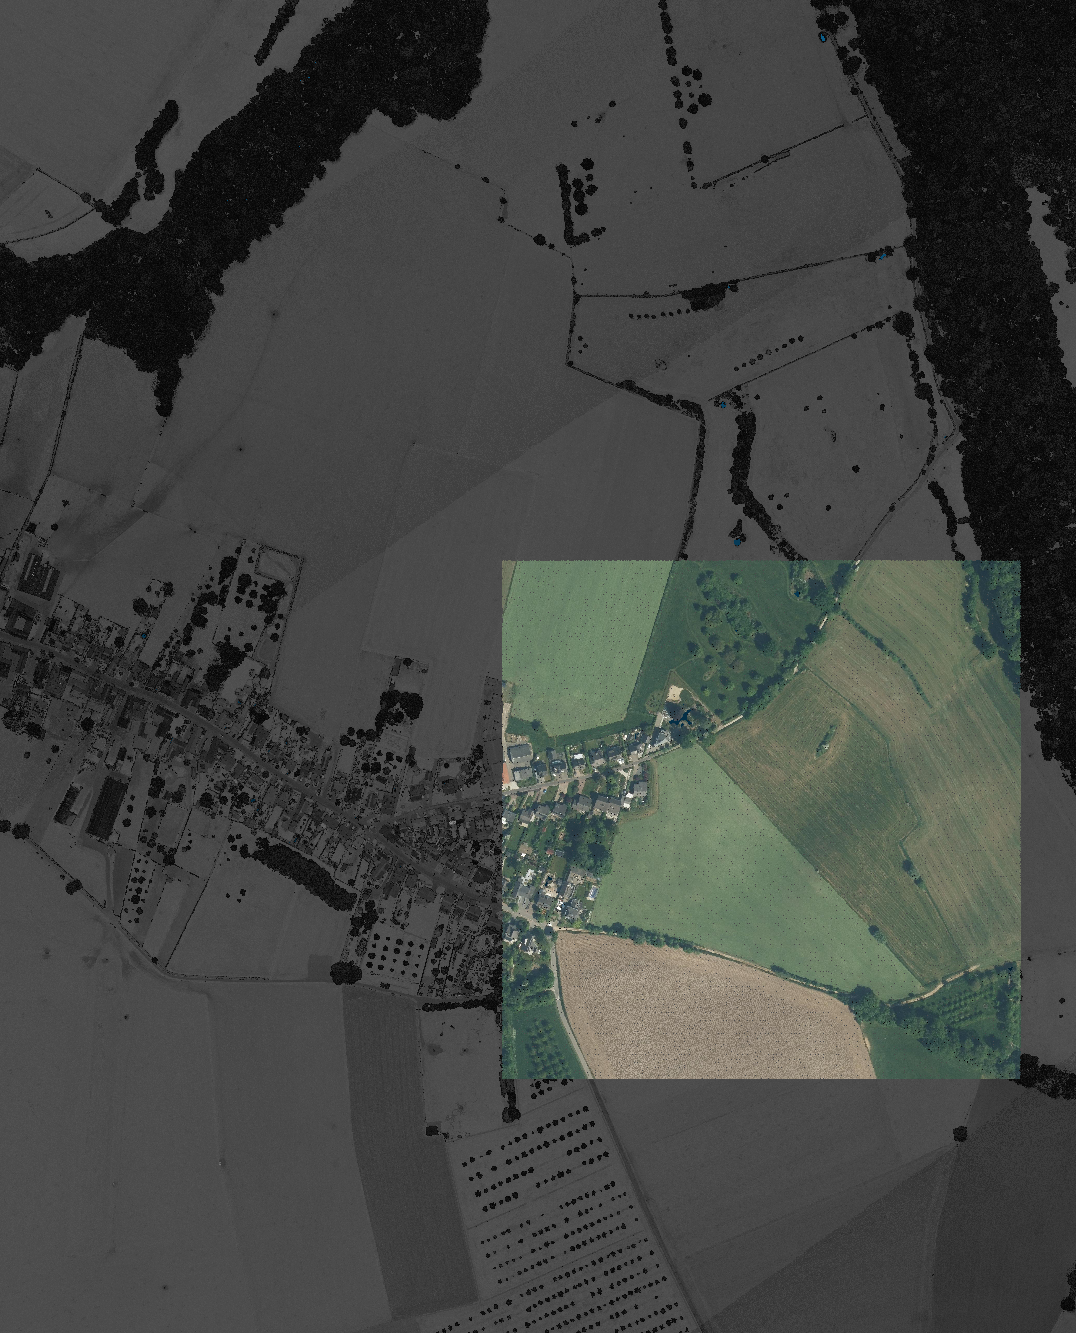
\includegraphics[width=0.5\linewidth]{img/screenshot_cropped_front.png}
  \caption{Clipped tile (500x500 meters) shown in RGB within context of full tile}
  \label{fig:cropped_front}
\end{figure}
The full and clipped tile are located in the EPSG:28992 coordinate system. The full tile spans from (186980, 314980) in the lower-left corner to (188020, 316270) in the top-right corner. The bounding box of the clipped tile ranges from (187466, 315228) in the lower-left corner to (187966, 315728) in the top-right corner.


Figure \ref{fig:cropped_elevation} shows some of this elevation, when looking at the clipped tile from the side using CloudCompare.

\begin{figure}[h]
  \centering
  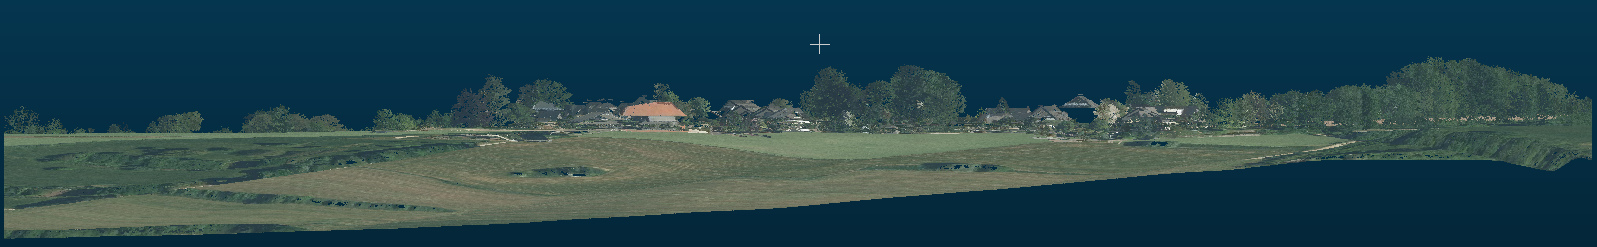
\includegraphics[width=0.5\linewidth]{img/screenshot_cropped_elevation.png}
  \caption{Side view of the cropped tile showcasing elevation}
  \label{fig:cropped_elevation}
\end{figure}
\newpage

In the first part of our C++ program, the tile cropping process is executed. The LAS file is read using the `lasreader.hpp` extension. The point cloud data is stored in a vector with the data type `Point3`, which is a CGAL data type. When reading the file, a thinning parameter, is passed to the read function. This parameter takes every nth point from the dataset, making sure the size of the data will be managable to work with. For now the thinning parameter is set to 1000, dividing the number of points of the dataset by the same amount.

Next, we specify the minimum and maximum x and y values by using the lower-left corner of the bounding box, as shown in the added figures above. Additionally, 500 meter is added to obtain the maximum x and y values.

\newpage

The C++ code snippet is as follows:

\begin{lstlisting}[style=cppstyle, caption={Specifying bounding box}, label={yourlabel}]
std::vector<Point3> lsPts = read_lasfile("../data/69BZ2_13.LAZ", 1000);

// Specify the bounding box of 500x500 meters
double min_x = 187465.5;
double max_x = min_x + 500;
double min_y = 315228.5;
double max_y = min_y + 500;

// extract points within bounding box
std::vector<Point3> filteredPts;
for (auto pt : lsPts) {
    if (pt.x() >= min_x && pt.x() <= max_x && pt.y() >= min_y && pt.y() <= max_y) {
      filteredPts.push_back(pt);
    }
  }
\end{lstlisting}
% Maybe this is not particularly necessary since we provide the code anyway,
% but I put it in for now; we can always delete it.

\section{Extract Ground and Create Gridded DTM}

Lorem ipsum dolor sit amet, consectetur adipiscing elit. Suspendisse id libero non arcu varius fermentum. Quisque malesuada nunc vel sapien vehicula, sit amet fringilla ligula aliquet. Nulla facilisi. Vivamus in ligula vitae arcu pellentesque rhoncus. Fusce eu elit nec mi fermentum sagittis. Integer id felis
\newpage

\section{Extract Vegetation Points and Create Grid}

Lorem ipsum dolor sit amet, consectetur adipiscing elit. Suspendisse id libero non arcu varius fermentum. Quisque malesuada nunc vel sapien vehicula, sit amet fringilla ligula aliquet. Nulla facilisi. Vivamus in ligula vitae arcu pellentesque rhoncus. Fusce eu elit nec mi fermentum sagittis. Integer id felis
\newpage

\section{Create the Canopy Height Model (CHM)}

Lorem ipsum dolor sit amet, consectetur adipiscing elit. Suspendisse id libero non arcu varius fermentum. Quisque malesuada nunc vel sapien vehicula, sit amet fringilla ligula aliquet. Nulla facilisi. Vivamus in ligula vitae arcu pellentesque rhoncus. Fusce eu elit nec mi fermentum sagittis. Integer id felis
\newpage

\section{References}


% ------------------------------------------------------------------------------

\end{document}
